\section{Theorie}
\label{sec:Theorie}

\subsection{Wirkungsweise}
\begin{figure}
 \centering
 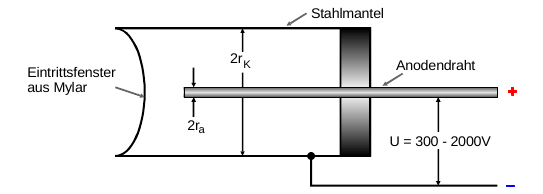
\includegraphics[width=\textwidth]{aufbaugeiger.png}
 \caption{Aufbau eines Geiger-Zählrohres.}
 \label{fig:aufn}
\end{figure}

Beim Geiger-Müller-Zählrohr umgibt ein Stahlmantel in zylindrischer Form
ein Gasgemisch, meist mit Alkoholanteil. Innen befindet sich ein Anodendraht,
dessen Gegenstück der Zylinder darstellt, der also auch als Kathode fungiert.\\
Geladene Teilchen tendieren dazu, stak zu reagieren, daher ist die wahrscheinlichkeit,
dass sie in das Innere des Zählrohrs eintreten, ausgesprochen gering. 
Stattdessen werden sie im metallischen Mantel absorbiert. Um dafür zu 
sorgen, dass auch einige Teilchen ins Innere gelangen, wird an die Seite,
die nicht mit dem Strom verbunden ist, eine dünne Wand aus Material mit Atomen
niedriger Ordnungszahl. Häufig wird beispielsweise Mylar-Folie verwendet. 
Diese Zählrohre werden auch Endfensterzählrohre genannt. Durch den im Zylinder
herrschenden Unterdruck beugt sich die Folie nach Innen, wie in \ref{fig:aufn} 
zu sehen ist.\\
Durch den zylindersymmetrischen Aufbau entsteht bei Anlegen einer äußeren Spannung
ein radialsymmetrisches Feld, für das gilt
\begin{equation}
\symup{E(r) }= \frac{U}{r ln\left(\frac{r_k}{r_a} \right) } 
\end{equation}
Wobei $r_a$ den Radius der Anode und $r_k$ den Radius der Kathode bezeichnen.
Ein geladenes Teilchen in diesem Feld wird um einen Wert beschleunigt, der
sich in einem Bereich von $\left( r_a < r < r_k \right)$ proportional zu $\frac{1}{r}$ 
verhält. \\
\\
Dringt ein geladenes Teilchen in das Zählrohr ein, wird seine Energie 
sich nach und nach durch Ionisation aufbrauchen, bis es vollständig absorbiert
ist. Die Energie, die das Teilchen zu Anfang hat, ist aber um ein Vielfaches
höher als die Energie pro gebildetem Ionenpaar, wodurch die Anzahl an 
entstehenden Elektronen und positiven Ionen proportional zur Anfangsenergie
ist. \\
Nach dieser Primärionisation laufen je nach angelegter Spannung verschiedene
Vorgänge ab.\\
Ist die Spannung gering, so erreichen nicht alle erzeugten Elektronen den Anodendraht
und die Anderen unterliegen vorher der Rekombination. In der Abbildung ist
dies der Bereich 1.\\
Als Ionisationskammer wird ein Gerät bezeichnet, das mit etwas höheren Spannungen
arbeitet, sodass die Rekombinationswahrscheinlichkeit weitaus geringer ist.
Es gelangen praktisch alle Elektronen zum Anodendraht und es fließt ein kontinuierlicher
Ionisationsstrom zwischen Kathode und Anode, der proportional zu Energie und
Intensität der einfallenden Strahlung ist. Bei weniger hohen Strahlintensitäten
ist der Einsatz einer Ionisationskammer nicht sinnvoll, da die entstehenden Ströme 
sehr klein sind.\\
Wenn die Spannung erhöht wird, steigt die Feldstärke in Drahtnähe, sodass die 
freigesetzten Elektronen ionisieren können, da sie zwischen den Zusammenstößen 
mit Argon-Atomen ausreichend Energie aufnehmen. Die durch diesen Stoßionisation genannten
Vorgang entstandenen Elektronen können auf dieselbe Weise wieder ionisieren,
solange die Spannung dazu aureicht, es bildet sich also eine sogenannte Townsend-Lawine
aus. \\
Pro einfallendem Teilchen sammelt sich nun so viel Ladung, dass ein Ladungsimpuls 
gemessen werden kann. Aufgrund des Proportionalitätszusammenhangs zwischen
gesammelter Ladung und Anfangsenergie ist dieser Ladungsimpuls ein Maß für 
die Teilchenenergie. Es wird in diesem Spannungsbereich daher von einem 
Proportionalzählrohr gesprochen.\\
Oberhalb dieses Proportionalbereichs ist die gesammelte Ladung unabhängig 
von der Anfangsenergie, allein das Volumen des Zählrohres und die Spannung sind
dann entscheidende Parameter. Durch die Elektronenlawinen werden Argon-Atome angeregt
und emittieren ultraviolette Photonen, wodurch dann wiederum 
freie Elektronen entstehen, aufgrund der Neutralität der Photonen im gesamten Volumen.
Es ist dann wieder nur die Intensität einfallender Strahlung messbar, nicht mehr
die Energie, allerdings arbeitet das Geiger-Müller-Zählrohr sehr viel effektiver als
das Proportionalzählrohr, da es einen geringeren elektronischen Aufwand verlangt.
Auch ist der Ladungsimpuls unabhängig vom Ionisationsvermögen der einfallenden Strahlung.

\subsection{Totzeit, Nachentladungen}
Als Totzeit T wird die Zeit bezeichnet, die das Geiger-Müller-Zählrohr nach
der Registrierung eines Teilchen nicht in der Lage ist, Weitere zu registrieren.
Sie ist eine Folge davon, dass die Ionen aufgrund ihrer Masse einige Zeit im
Gasgemisch zwischen Kathode und Anode bleiben, während die leichteren Elektronen
schnell zur Anode in der Mitte wandern. So entsteht eine positive Ladung im 
Zylinder, auch Ionenschlauch genannt, die die Feldstärke um den Draht herabsetzt.
In dieser Zeit ist dann keine Stoßionisation möglich.\\
Durch ihre positive Ladung wandert die Ionenwolke zum Zylindermantel, der Kathode
der Anordnung. Dabei kann die Feldstärke ansteigen und Lawinenbildung wieder ermöglichen.
Die dadurch entstehenden Signale werden aber schwächer sein, bis die Feldstärke
wieder ihren ursprünglichen Wert erreicht hat, also auch die Ionen aller nachfolgenden
Prozesse neutralisiert wurden. Diese Zeit, die sich unmittelbar an die Totzeit
anschließt, wird Erholungszeit $T_E$ genannt.\\
\\
\begin{figure}
 \centering
 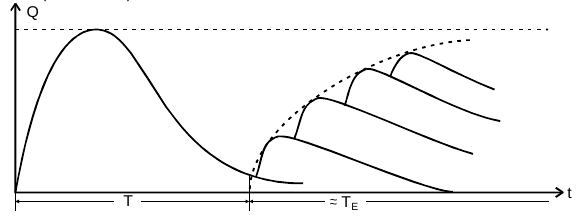
\includegraphics[width=\textwidth]{zeitengeiger.png}
 \caption{Beispielhafte Darstellung von Tot- und Erholungszeit.}
 \label{fig:gramm}
\end{figure}
In Abbildung \ref{fig:gramm} werden diese beiden Zeiträume qualitativ dargestellt.\\
Treffen die zuvor beschriebenen Ionen dann auf den Mantel, können sie aus dem
Metall Elektronen herauslösen, die dann die Zählrohrentladung erneut zünden können.
Sie werden als Sekundärelektronen bezeichnet und sorgen dafür, dass ein einzelnes
Teilchen mehrere Ausgangsimpulse zur Folge haben kann: Die Primärentladung und
weitere Nachentladungen, die im Abstand von der Laufzeit $T_L$ der Ionen 
auftreten. Im Allgemeinen ist diese Laufzeit größer als die Totzeit, wodurch es
scheint, als würden weitere ionisierte Teilchen das Rohr durchqueren.\\
Es ist also eine wichtige Aufgabe, diese Nachentladung mögllichst zu unterbinden.
Dazu wird der Alkoholanteil im Gasgemisch nützlich: Die Edelgasionen 
ionisieren durch Zusammenstöße die Alkoholmoleküle, und da deren Energie 
geringer ist, reicht sie bein Auftreffen auf den Zylindermantel nicht aus,
um Elektronen herauszulösen. 

\subsection{Charakteristik}
\begin{figure}
 \centering
 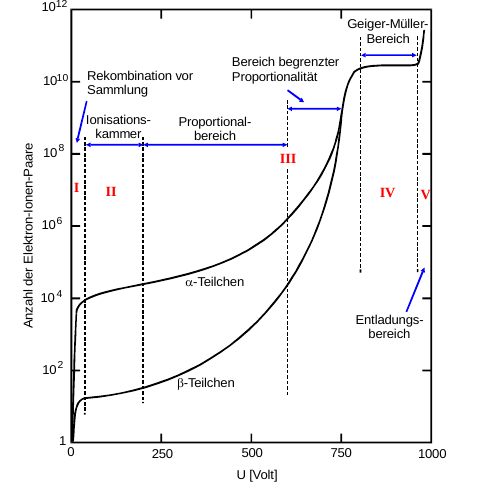
\includegraphics[width=\textwidth]{kurvegeiger.png}
 \caption{Charakteristik eines Geiger-Müller-Zählrohres.}
 \label{fig:char}
\end{figure}

Als Charakteristik eines Geiger-Müller-Zählrohrs bezeichnet man ein Diagramm,
in dem die registrierte Teilchenzahl gegen die angelegte Spannung aufgetragen wird.
Dabei soll die Strahlungsintensität konstant bleiben. Abbildung \ref{fig:char} zeigt 
ein Beispiel einer solchen Charakteristik.\\
$U_E$ markiert den Zeitpunkt, an dem der Auslösebereich beginnt. Der darauf
folgende, Plateau genannte, Bereich verläuft linear. Idealerweise sollte die 
Steigung null sein, real ist das allerdings nicht zu erreichen, da bei steigender
Spannung auch die Teilchenzahl gering steigen wird, wegen Nachladungen, die
die Alkoholdämpfe nicht verhindern können. Die Steigung des Plateaus ist auch ein
Indikator für die Qualität des Zählrohrs; Je geringer sie ist, desto größer
die Qualität.\\
Nach dem Plateau folgt ein Bereich mit großer Anzahl an Nachentladungen, die in den
Bereich der selbstständigen Gasentladung übergeht. Dabei löst ein einziges Teilchen 
eine Dauerentladung aus, was fatale Auswirkung auf das Zählrohr haben kann.\\

\subsection{Ansprechvermögen}
Ein weiterer wichtiger Begriff im Zusammenhang mit Geiger-Müller-Zählrohren 
ist das Ansprechvermögen.
Er wird in Prozent angegeben und bezeichnet die Wahrscheinlichkeit, dass ein Teilchen im Zählrohr nachgewiesen
wird. Geladene Teilchen wie $\alpha$- oder $\beta$-Teilchen haben typischerweise ein höheres Ansprechvermögen, 
da sie reaktionsfreudiger sind als ungeladene Photonen. Daher kann ein
Geiger-Müller-Zählrohr nur sinnvoll eingesetzt werden, wenn die Intensität
der Photonen sehr hoch ist. Für niederenergetischere Photonen könnte allerdings
ein schwereres Füllgas verwendet werden.

\subsection{Bestimmung der Totzeit über die Zwei-Quellen-Methode}
Durch die zuvor beschriebene Totzeit wird die aufgenommene Impulsrate immer
kleiner sein als die tatsächliche Anzahl der Teilchen, die das Volumen durchquert haben.
Treffen während einer Messung $N_r$ Teilchen ein, so ist $TN_r$ der Bruchteil
der gesamten Messzeit, in dem keine weiteren Teilchen gemessen werden können.
Also werden im $1 - TN_r$ -Teil der Messzeit alle Teilchen gemessen.\\
Es gilt dann für die wahre Impulsrate
\begin{equation}
N_w = \frac{N_r t}{\left( 1 - TN_r \right) t} = \frac{N_r}{1 - TN_r}
\end{equation}
Indem zwei verschiedene Präparate genutzt werden und die Impulsraten für beide
gemessen werden, genau wie die Impulsrate für beide Präparate zusammen, lässt sich
die Totzeit bestimmen. \\
Ohne sie würde gelten
\begin{equation}
N_{1+2} = N_1 + N_2
\end{equation}
Doch es wird gemessen, dass
\begin{equation}
N_{1+2} < N_1 + N_2
\end{equation}
Für die wahren Impulsraten der Messungen gelten
\begin{align}
N_{w_1} = \frac{N_1}{1 - TN_1}\\
N_{w_2} = \frac{N_2}{1 - TN_2}\\
N_{w_{1+2}} = \frac{N_{1+2}}{1 - TN_{1+2}}
\end{align}
Die wahren Impulsraten müssen aber $N_{w_{1+2}} = N_{w_1} + N_{w_2}$ gehorchen, sodass
\begin{equation}
\frac{N_{1+2}}{1 - TN_{1+2}} = \frac{N_1}{1 - TN_1} + \frac{N_2}{1 - TN_2}
\end{equation}
Unter der Bedingung, dass $T^2  N^2_i << 1$ gilt, lässt sich T näherungsweise 
aus dieser Formel zu 
\begin{equation}
T \approx \frac{N_1 + N_2 - N_{1+2}}{2N_1 N_2}
\end{equation}
bestimmen. 
